\chapter{Game theory}

In this chapter, we will focus on games where
two players make alternate moves and that 
do not contain random elements.
Our goal is to find a strategy that we can
follow to win the game
no matter what the opponent does,
if such a strategy exists.

It turns out that there is a general strategy
for all such games,
and we can analyze the games using the \key{nim theory}.
First, we analyze simple games where
players remove sticks from heaps,
and after this, we generalize the strategy
for those games to all other games.

\section{Game states}

Let's consider a game where there is initially
a heap of $n$ sticks.
Players $A$ and $B$ move alternatively,
and player $A$ begins.
On each move, the player has to remove
1, 2 or 3 sticks from the heap.
The player who removes the last stick wins.

For example, if $n=10$, the game may proceed as follows:
\begin{enumerate}[noitemsep]
\item Player $A$ removes 2 sticks (8 sticks left).
\item Player $B$ removes 3 sticks (5 sticks left).
\item Player $A$ removes 1 stick (4 sticks left).
\item Player $B$ removes 2 sticks (2 sticks left).
\item Player $A$ removes 2 sticks and wins.
\end{enumerate}
This game consists of states $0,1,2,\ldots,n$,
where the number of the state corresponds to
the number of sticks left.
The player must always choose how many sticks
they will remove from the heap.

\subsubsection{Winning and losing states}

\index{winning state}
\index{losing state}

A \key{winning state} is a state where
the player wins the game if they
play optimally.
Correspondingly, a \key{losing state} is a state
where the player loses if the
opponent plays optimally.
It turns out that we can classify all states
in a game so that each state is either
a winning state or a losing state.

In the above game, state 0 is clearly a
losing state, because the player can't make
any moves.
States 1, 2 and 3 are winning states,
because we can remove 1, 2 or 3 sticks
and win the game.
State 4, in turn, is a losing state,
because any move leads to a state that
is a winning state for the opponent.

More generally, if there is a move that leads
from the current state to a losing state,
the current state is a winning state,
and otherwise it is a losing state.
Using this observation, we can classify all states
in a game beginning from losing states where
there are no possible moves.

The states $0 \ldots 15$ of the above game
can be classified as follows
($W$ means winning state, and $L$ means losing state):
\begin{center}
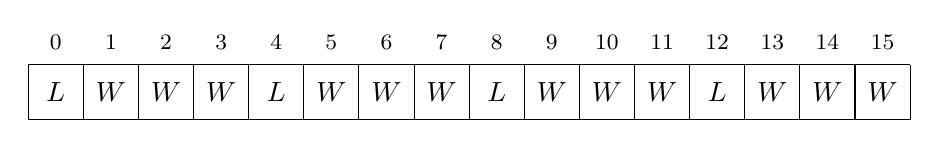
\begin{tikzpicture}[scale=0.7]
\draw (0,0) grid (16,1);

\node at (0.5,0.5) {$L$};
\node at (1.5,0.5) {$W$};
\node at (2.5,0.5) {$W$};
\node at (3.5,0.5) {$W$};
\node at (4.5,0.5) {$L$};
\node at (5.5,0.5) {$W$};
\node at (6.5,0.5) {$W$};
\node at (7.5,0.5) {$W$};
\node at (8.5,0.5) {$L$};
\node at (9.5,0.5) {$W$};
\node at (10.5,0.5) {$W$};
\node at (11.5,0.5) {$W$};
\node at (12.5,0.5) {$L$};
\node at (13.5,0.5) {$W$};
\node at (14.5,0.5) {$W$};
\node at (15.5,0.5) {$W$};

\footnotesize
\node at (0.5,1.4) {$0$};
\node at (1.5,1.4) {$1$};
\node at (2.5,1.4) {$2$};
\node at (3.5,1.4) {$3$};
\node at (4.5,1.4) {$4$};
\node at (5.5,1.4) {$5$};
\node at (6.5,1.4) {$6$};
\node at (7.5,1.4) {$7$};
\node at (8.5,1.4) {$8$};
\node at (9.5,1.4) {$9$};
\node at (10.5,1.4) {$10$};
\node at (11.5,1.4) {$11$};
\node at (12.5,1.4) {$12$};
\node at (13.5,1.4) {$13$};
\node at (14.5,1.4) {$14$};
\node at (15.5,1.4) {$15$};
\end{tikzpicture}
\end{center}

It's easy to analyze this game:
a state $k$ is a losing state if $k$ is
divisible by 4, and otherwise it
is winning state.
An optimal way to play the game is
to always choose a move after which
the number of sticks in the heap
is divisible by 4.
Finally, there are no sticks left and
the opponent has lost.

Of course, this strategy requires that
the number of sticks is \emph{not} divisible by 4
when it is our move.
If it is, there is nothing we can do,
but the opponent will win the game if
they play optimally.

\subsubsection{State graph}

Let's now consider another stick game,
where in state $k$, it is allowed to remove
any number $x$ of sticks such that $x$
is smaller than $x$ and divides $x$.
For example, in state 8 we may remove
1, 2 or 4 sticks, but in state 7 the only
allowed move is to remove 1 stick.

The following picture shows the states
$1 \ldots 9$ of the game as a \key{state graph},
where nodes are states and edges are moves between them:

\begin{center}
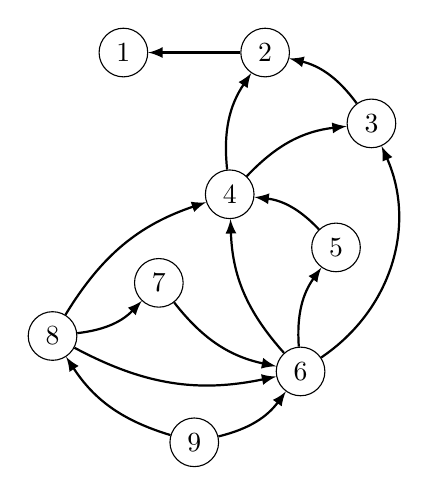
\begin{tikzpicture}[scale=0.9]
\node[draw, circle] (1) at (0,0) {$1$};
\node[draw, circle] (2) at (2,0) {$2$};
\node[draw, circle] (3) at (3.5,-1) {$3$};
\node[draw, circle] (4) at (1.5,-2) {$4$};
\node[draw, circle] (5) at (3,-2.75) {$5$};
\node[draw, circle] (6) at (2.5,-4.5) {$6$};
\node[draw, circle] (7) at (0.5,-3.25) {$7$};
\node[draw, circle] (8) at (-1,-4) {$8$};
\node[draw, circle] (9) at (1,-5.5) {$9$};

\path[draw,thick,->,>=latex] (2) -- (1);
\path[draw,thick,->,>=latex] (3) edge [bend right=20] (2);
\path[draw,thick,->,>=latex] (4) edge [bend left=20] (2);
\path[draw,thick,->,>=latex] (4) edge [bend left=20] (3);
\path[draw,thick,->,>=latex] (5) edge [bend right=20] (4);
\path[draw,thick,->,>=latex] (6) edge [bend left=20] (5);
\path[draw,thick,->,>=latex] (6) edge [bend left=20] (4);
\path[draw,thick,->,>=latex] (6) edge [bend right=40] (3);
\path[draw,thick,->,>=latex] (7) edge [bend right=20] (6);
\path[draw,thick,->,>=latex] (8) edge [bend right=20] (7);
\path[draw,thick,->,>=latex] (8) edge [bend right=20] (6);
\path[draw,thick,->,>=latex] (8) edge [bend left=20] (4);
\path[draw,thick,->,>=latex] (9) edge [bend left=20] (8);
\path[draw,thick,->,>=latex] (9) edge [bend right=20] (6);
\end{tikzpicture}
\end{center}

The final state in this game is always state 1,
which is a losing state, because there are no
valid moves.
The classification of states $1 \ldots 9$
is as follows:

\begin{center}
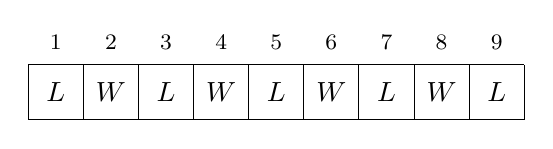
\begin{tikzpicture}[scale=0.7]
\draw (1,0) grid (10,1);

\node at (1.5,0.5) {$L$};
\node at (2.5,0.5) {$W$};
\node at (3.5,0.5) {$L$};
\node at (4.5,0.5) {$W$};
\node at (5.5,0.5) {$L$};
\node at (6.5,0.5) {$W$};
\node at (7.5,0.5) {$L$};
\node at (8.5,0.5) {$W$};
\node at (9.5,0.5) {$L$};

\footnotesize
\node at (1.5,1.4) {$1$};
\node at (2.5,1.4) {$2$};
\node at (3.5,1.4) {$3$};
\node at (4.5,1.4) {$4$};
\node at (5.5,1.4) {$5$};
\node at (6.5,1.4) {$6$};
\node at (7.5,1.4) {$7$};
\node at (8.5,1.4) {$8$};
\node at (9.5,1.4) {$9$};
\end{tikzpicture}
\end{center}

Surprisingly enough, in this game,
all even-numbered states are winning states,
and all odd-numbered states are losing states.

\section{Nim game}

\index{nim game}

The \key{nim game} is a simple game that
has an important role in game theory,
because many games can be played using
the same strategy.
First, we focus on nim,
and then we generalize the strategy
to other games.

There are $n$ heaps in nim,
and each heap contains some number of sticks.
The players move alternatively,
and on each turn, the player chooses
a heap that still contains sticks
and removes any number of sticks from it.
The winner is the player who removes the last stick.

The states in nim are of the form
$[x_1,x_2,\ldots,x_n]$,
where $x_k$ denotes the number of sticks in heap $k$.
For example, $[10,12,5]$ is a game where
there are three heaps with 10, 12 and 5 sticks.
The state $[0,0,\ldots,0]$ is a losing state,
because it's not possible to remove any sticks,
and this is always the final state.

\subsubsection{Analysis}
\index{nim sum}

It turns out that we can easily find out
the type of any nim state by calculating
a \key{nim sum} $x_1 \oplus x_2 \oplus \cdots \oplus x_n$,
where $\oplus$ is the xor operation.
The states with nim sum 0 are losing states,
and all other states are winning states.
For example, the nim sum for
$[10,12,5]$ is $10 \oplus 12 \oplus 5 = 3$,
so the state is a winning state.

But how is the nim sum related to the nim game?
We can explain this by studying how the nim
sum changes when the nim state changes.

~\\
\noindent
\textit{Losing states:}
The final state $[0,0,\ldots,0]$ is a losing state,
and its nim sum is 0, as expected.
In other losing states, any move leads to
a winning state, because when a single value $x_k$ changes,
the nim sum also changes, so the nim sum
is different from 0 after the move.

~\\
\noindent
\textit{Winning states:}
We can move to a losing state if
there is any heap $k$ for which $x_k \oplus s < x_k$.
In this case, we can remove sticks from
heap $k$ so that it will contain $x_k \oplus s$ sticks,
which will lead to a losing state.
There is always such a heap, where $x_k$
has a one bit in position of the leftmost
one bit in $s$.

~\\
\noindent
As an example, let's consider the state $[10,2,5]$.
This state is a winning state,
because its nim sum is 3.
Thus, there has to be a move which
leads to a losing state.
Next we will find out such a move.

\begin{samepage}
The nim sum of the state is as follows:

\begin{center}
\begin{tabular}{r|r}
10 & \texttt{1010} \\
12 & \texttt{1100} \\
5 & \texttt{0101} \\
\hline
3 & \texttt{0011} \\
\end{tabular}
\end{center}
\end{samepage}

In this case, the heap with 10 sticks
is the only heap that has a one bit
in the position of the leftmost
one bit in the nim sum:

\begin{center}
\begin{tabular}{r|r}
10 & \texttt{10\textcircled{1}0} \\
12 & \texttt{1100} \\
5 & \texttt{0101} \\
\hline
3 & \texttt{00\textcircled{1}1} \\
\end{tabular}
\end{center}

The new size of the heap has to be
$10 \oplus 3 = 9$,
so we will remove just one stick.
After this, the state will be $[9,12,5]$,
which is a losing state:

\begin{center}
\begin{tabular}{r|r}
9 & \texttt{1001} \\
12 & \texttt{1100} \\
5 & \texttt{0101} \\
\hline
0 & \texttt{0000} \\
\end{tabular}
\end{center}

\subsubsection{Misère game}

\index{misère game}

In a \key{misère game}, the goal is opposite,
so the player who removes the last stick
loses the game.
It turns out that a misère nim game can be
optimally played almost like the standard nim game.

The idea is to first play the misère game
like a standard game, but change the strategy
at the end of the game.
The new strategy will be used when after the next move,
each heap would contain at most one stick.

In the standard game, we should choose a move
after which there is an even number of heaps with one stick.
However, in the misère game, we choose a move so that
there is an odd number of heaps with one stick.

This strategy works because the state where the
strategy changes always appears in a game,
and this state is a winning state, because
it contains exactly one heap that has more than one stick,
so the nim sum is not 0.

\section{Sprague–Grundyn lause}

\index{Sprague–Grundyn lause}

\key{Sprague–Grundyn lause} yleistää nim-pelin strategian
kaikkiin peleihin, jotka täyttävät
seuraavat vaatimukset:

\begin{itemize}[noitemsep]
\item Pelissä on kaksi pelaajaa, jotka tekevät vuorotellen siirtoja.
\item Peli muodostuu tiloista ja mahdolliset siirrot tilasta
eivät riipu siitä, kumpi pelaaja on vuorossa.
\item Peli päättyy, kun toinen pelaaja ei voi tehdä siirtoa.
\item Peli päättyy varmasti ennemmin tai myöhemmin.
\item Pelaajien saatavilla on kaikki tieto tiloista
ja siirroista, eikä pelissä ole satunnaisuutta.
\end{itemize}
Ideana on laskea kullekin pelin tilalle Grundy-luku,
joka vastaa tikkujen määrää nim-pelin kasassa.
Kun kaikkien tilojen Grundy-luvut ovat tiedossa,
peliä voi pelata aivan kuin se olisi nim-peli.

\subsubsection{Grundy-luku}

\index{Grundy-luku}
\index{mex-funktio}

Pelin tilan \key{Grundy-luku} määritellään rekursiivisesti
kaavalla
\[\textrm{mex}(\{g_1,g_2,\ldots,g_n\}),\]
jossa $g_1,g_2,\ldots,g_n$ ovat niiden tilojen
Grundy-luvut, joihin tilasta pääsee yhdellä siirrolla,
ja funktio mex antaa pienimmän ei-negatiivisen
luvun, jota ei esiinny joukossa.
Esimerkiksi $\textrm{mex}(\{0,1,3\})=2$.
Jos tilasta ei voi tehdä mitään siirtoa,
sen Grundy-luku on 0, koska $\textrm{mex}(\emptyset)=0$.

Esimerkiksi tilaverkossa
\begin{center}
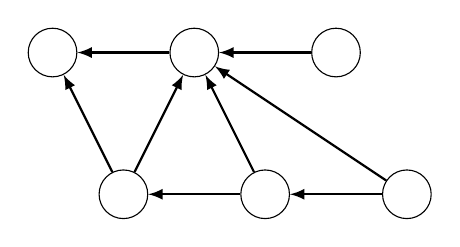
\begin{tikzpicture}[scale=0.9]
\node[draw, circle] (1) at (0,0) {\phantom{0}};
\node[draw, circle] (2) at (2,0) {\phantom{0}};
\node[draw, circle] (3) at (4,0) {\phantom{0}};
\node[draw, circle] (4) at (1,-2) {\phantom{0}};
\node[draw, circle] (5) at (3,-2) {\phantom{0}};
\node[draw, circle] (6) at (5,-2) {\phantom{0}};

\path[draw,thick,->,>=latex] (2) -- (1);
\path[draw,thick,->,>=latex] (3) -- (2);
\path[draw,thick,->,>=latex] (5) -- (4);
\path[draw,thick,->,>=latex] (6) -- (5);
\path[draw,thick,->,>=latex] (4) -- (1);
\path[draw,thick,->,>=latex] (4) -- (2);
\path[draw,thick,->,>=latex] (5) -- (2);
\path[draw,thick,->,>=latex] (6) -- (2);
\end{tikzpicture}
\end{center}
Grundy-luvut ovat seuraavat:
\begin{center}
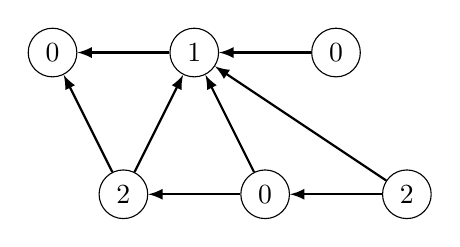
\begin{tikzpicture}[scale=0.9]
\node[draw, circle] (1) at (0,0) {0};
\node[draw, circle] (2) at (2,0) {1};
\node[draw, circle] (3) at (4,0) {0};
\node[draw, circle] (4) at (1,-2) {2};
\node[draw, circle] (5) at (3,-2) {0};
\node[draw, circle] (6) at (5,-2) {2};

\path[draw,thick,->,>=latex] (2) -- (1);
\path[draw,thick,->,>=latex] (3) -- (2);
\path[draw,thick,->,>=latex] (5) -- (4);
\path[draw,thick,->,>=latex] (6) -- (5);
\path[draw,thick,->,>=latex] (4) -- (1);
\path[draw,thick,->,>=latex] (4) -- (2);
\path[draw,thick,->,>=latex] (5) -- (2);
\path[draw,thick,->,>=latex] (6) -- (2);
\end{tikzpicture}
\end{center}
Jos tila on häviötila, sen Grundy-luku on 0.
Jos taas tila on voittotila, sen Grundy-luku
on jokin positiivinen luku.

Grundy-luvun hyötynä on,
että se vastaa tikkujen määrää nim-kasassa.
Jos Grundy-luku on 0, niin tilasta pääsee vain tiloihin,
joiden Grundy-luku ei ole 0.
Jos taas Grundy-luku on $x>0$, niin tilasta pääsee tiloihin,
joiden Grundy-luvut kattavat välin $0,1,\ldots,x-1$.

~\\
\noindent
Tarkastellaan esimerkkinä peliä,
jossa pelaajat siirtävät vuorotellen
pelihahmoa sokkelossa.
Jokainen sokkelon ruutu on lattiaa tai seinää.
Kullakin siirrolla hahmon tulee liikkua jokin
määrä askeleita vasemmalle tai jokin
määrä askeleita ylöspäin.
Pelin voittaja on se, joka tekee viimeisen siirron.

\begin{samepage}
Esimerkiksi seuraavassa on pelin mahdollinen aloitustilanne,
jossa @ on pelihahmo ja * merkitsee ruutua, johon hahmo voi siirtyä.

\begin{center}
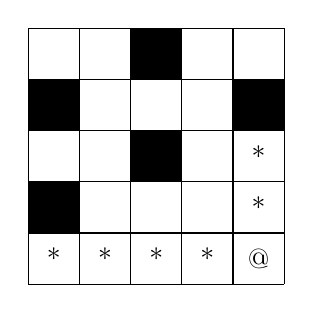
\begin{tikzpicture}[scale=.65]
  \begin{scope}
    \fill [color=black] (0, 1) rectangle (1, 2);
    \fill [color=black] (0, 3) rectangle (1, 4);
    \fill [color=black] (2, 2) rectangle (3, 3);
    \fill [color=black] (2, 4) rectangle (3, 5);
    \fill [color=black] (4, 3) rectangle (5, 4);

    \draw (0, 0) grid (5, 5);
    
    \node at (4.5,0.5) {@};
    \node at (3.5,0.5) {*};
    \node at (2.5,0.5) {*};
    \node at (1.5,0.5) {*};
    \node at (0.5,0.5) {*};
    \node at (4.5,1.5) {*};
    \node at (4.5,2.5) {*};
    
  \end{scope}
\end{tikzpicture}
\end{center}
\end{samepage}

Sokkelopelin tiloja ovat kaikki sokkelon
lattiaruudut. Tässä tapauksessa
tilojen Grundy-luvut ovat seuraavat:

\begin{center}
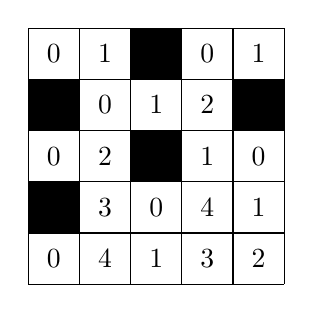
\begin{tikzpicture}[scale=.65]
  \begin{scope}
    \fill [color=black] (0, 1) rectangle (1, 2);
    \fill [color=black] (0, 3) rectangle (1, 4);
    \fill [color=black] (2, 2) rectangle (3, 3);
    \fill [color=black] (2, 4) rectangle (3, 5);
    \fill [color=black] (4, 3) rectangle (5, 4);

    \draw (0, 0) grid (5, 5);
    
    \node at (0.5,4.5) {0};
    \node at (1.5,4.5) {1};
    \node at (2.5,4.5) {};
    \node at (3.5,4.5) {0};
    \node at (4.5,4.5) {1};

    \node at (0.5,3.5) {};
    \node at (1.5,3.5) {0};
    \node at (2.5,3.5) {1};
    \node at (3.5,3.5) {2};
    \node at (4.5,3.5) {};

    \node at (0.5,2.5) {0};
    \node at (1.5,2.5) {2};
    \node at (2.5,2.5) {};
    \node at (3.5,2.5) {1};
    \node at (4.5,2.5) {0};

    \node at (0.5,1.5) {};
    \node at (1.5,1.5) {3};
    \node at (2.5,1.5) {0};
    \node at (3.5,1.5) {4};
    \node at (4.5,1.5) {1};

    \node at (0.5,0.5) {0};
    \node at (1.5,0.5) {4};
    \node at (2.5,0.5) {1};
    \node at (3.5,0.5) {3};
    \node at (4.5,0.5) {2};
  \end{scope}
\end{tikzpicture}
\end{center}

Tämän seurauksena sokkelopelin
tila käyttäytyy
samalla tavalla kuin nim-pelin kasa.
Esimerkiksi oikean alakulman ruudun
Grundy-luku on 2,
joten kyseessä on voittotila.
Voittoon johtava siirto on joko liikkua neljä
askelta vasemmalle tai kaksi askelta ylöspäin.

Huomaa, että toisin kuin alkuperäisessä nim-pelissä,
tilasta saattaa päästä toiseen tilaan,
jonka Grundy-luku on suurempi.
Vastustaja voi kuitenkin aina peruuttaa
tällaisen siirron niin,
että Grundy-luku palautuu samaksi.

\subsubsection{Alipelit}

Oletetaan seuraavaksi, että peli muodostuu
alipeleistä ja jokaisella vuorolla
pelaaja valitsee jonkin alipeleistä ja
tekee siirron siinä.
Peli päättyy, kun missään alipelissä ei
pysty tekemään siirtoa.

Nyt pelin tilan Grundy-luku on alipelien
Grundy-lukujen nim-summa.
Peliä pystyy pelaamaan nim-pelin
tapaan selvittämällä kaikkien alipelien Grundy-luvut
ja laskemalla niiden nim-summa.

~\\
\noindent
Tarkastellaan esimerkkinä kolmen sokkelon peliä.
Tässä pelissä pelaaja valitsee joka siirrolla
yhden sokkeloista ja siirtää siinä olevaa hahmoa.
Pelin aloitustilanne voi olla seuraavanlainen:

\begin{center}
\begin{tabular}{ccc}
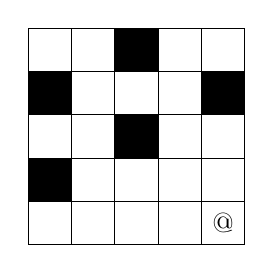
\begin{tikzpicture}[scale=.55]
  \begin{scope}
    \fill [color=black] (0, 1) rectangle (1, 2);
    \fill [color=black] (0, 3) rectangle (1, 4);
    \fill [color=black] (2, 2) rectangle (3, 3);
    \fill [color=black] (2, 4) rectangle (3, 5);
    \fill [color=black] (4, 3) rectangle (5, 4);

    \draw (0, 0) grid (5, 5);

    \node at (4.5,0.5) {@};

    \end{scope}
\end{tikzpicture}
&
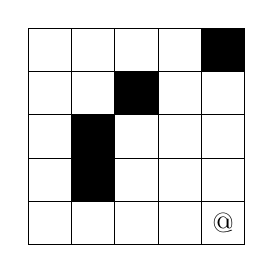
\begin{tikzpicture}[scale=.55]
  \begin{scope}
    \fill [color=black] (1, 1) rectangle (2, 3);
    \fill [color=black] (2, 3) rectangle (3, 4);
    \fill [color=black] (4, 4) rectangle (5, 5);

    \draw (0, 0) grid (5, 5);
    
    \node at (4.5,0.5) {@};

  \end{scope}
\end{tikzpicture}
&
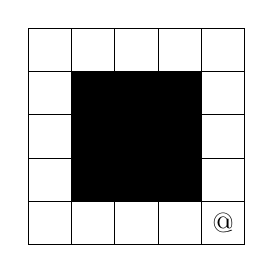
\begin{tikzpicture}[scale=.55]
  \begin{scope}
    \fill [color=black] (1, 1) rectangle (4, 4);

    \draw (0, 0) grid (5, 5);
    
    \node at (4.5,0.5) {@};
  \end{scope}
\end{tikzpicture}
\end{tabular}
\end{center}

Sokkeloiden ruutujen Grundy-luvut ovat:

\begin{center}
\begin{tabular}{ccc}
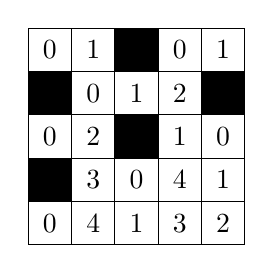
\begin{tikzpicture}[scale=.55]
  \begin{scope}
    \fill [color=black] (0, 1) rectangle (1, 2);
    \fill [color=black] (0, 3) rectangle (1, 4);
    \fill [color=black] (2, 2) rectangle (3, 3);
    \fill [color=black] (2, 4) rectangle (3, 5);
    \fill [color=black] (4, 3) rectangle (5, 4);

    \draw (0, 0) grid (5, 5);

    \node at (0.5,4.5) {0};
    \node at (1.5,4.5) {1};
    \node at (2.5,4.5) {};
    \node at (3.5,4.5) {0};
    \node at (4.5,4.5) {1};

    \node at (0.5,3.5) {};
    \node at (1.5,3.5) {0};
    \node at (2.5,3.5) {1};
    \node at (3.5,3.5) {2};
    \node at (4.5,3.5) {};

    \node at (0.5,2.5) {0};
    \node at (1.5,2.5) {2};
    \node at (2.5,2.5) {};
    \node at (3.5,2.5) {1};
    \node at (4.5,2.5) {0};

    \node at (0.5,1.5) {};
    \node at (1.5,1.5) {3};
    \node at (2.5,1.5) {0};
    \node at (3.5,1.5) {4};
    \node at (4.5,1.5) {1};

    \node at (0.5,0.5) {0};
    \node at (1.5,0.5) {4};
    \node at (2.5,0.5) {1};
    \node at (3.5,0.5) {3};
    \node at (4.5,0.5) {2};
    \end{scope}
\end{tikzpicture}
&
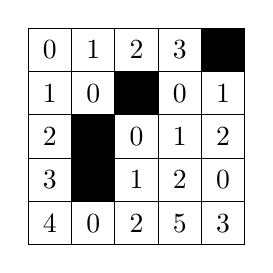
\begin{tikzpicture}[scale=.55]
  \begin{scope}
    \fill [color=black] (1, 1) rectangle (2, 3);
    \fill [color=black] (2, 3) rectangle (3, 4);
    \fill [color=black] (4, 4) rectangle (5, 5);

    \draw (0, 0) grid (5, 5);

    \node at (0.5,4.5) {0};
    \node at (1.5,4.5) {1};
    \node at (2.5,4.5) {2};
    \node at (3.5,4.5) {3};
    \node at (4.5,4.5) {};

    \node at (0.5,3.5) {1};
    \node at (1.5,3.5) {0};
    \node at (2.5,3.5) {};
    \node at (3.5,3.5) {0};
    \node at (4.5,3.5) {1};

    \node at (0.5,2.5) {2};
    \node at (1.5,2.5) {};
    \node at (2.5,2.5) {0};
    \node at (3.5,2.5) {1};
    \node at (4.5,2.5) {2};

    \node at (0.5,1.5) {3};
    \node at (1.5,1.5) {};
    \node at (2.5,1.5) {1};
    \node at (3.5,1.5) {2};
    \node at (4.5,1.5) {0};

    \node at (0.5,0.5) {4};
    \node at (1.5,0.5) {0};
    \node at (2.5,0.5) {2};
    \node at (3.5,0.5) {5};
    \node at (4.5,0.5) {3};
  \end{scope}
\end{tikzpicture}
&
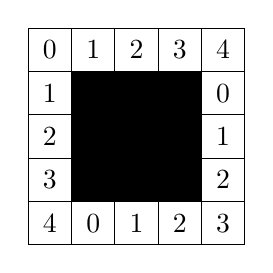
\begin{tikzpicture}[scale=.55]
  \begin{scope}
    \fill [color=black] (1, 1) rectangle (4, 4);

    \draw (0, 0) grid (5, 5);

    \node at (0.5,4.5) {0};
    \node at (1.5,4.5) {1};
    \node at (2.5,4.5) {2};
    \node at (3.5,4.5) {3};
    \node at (4.5,4.5) {4};

    \node at (0.5,3.5) {1};
    \node at (1.5,3.5) {};
    \node at (2.5,3.5) {};
    \node at (3.5,3.5) {};
    \node at (4.5,3.5) {0};

    \node at (0.5,2.5) {2};
    \node at (1.5,2.5) {};
    \node at (2.5,2.5) {};
    \node at (3.5,2.5) {};
    \node at (4.5,2.5) {1};

    \node at (0.5,1.5) {3};
    \node at (1.5,1.5) {};
    \node at (2.5,1.5) {};
    \node at (3.5,1.5) {};
    \node at (4.5,1.5) {2};

    \node at (0.5,0.5) {4};
    \node at (1.5,0.5) {0};
    \node at (2.5,0.5) {1};
    \node at (3.5,0.5) {2};
    \node at (4.5,0.5) {3};
  \end{scope}
\end{tikzpicture}
\end{tabular}
\end{center}

Aloitustilanteessa Grundy-lukujen nim-summa on
$2 \oplus 3 \oplus 3 = 2$, joten
aloittaja pystyy voittamaan pelin.
Voittoon johtava siirto on liikkua vasemmassa sokkelossa
2 askelta ylöspäin, jolloin nim-summaksi
tulee $0 \oplus 3 \oplus 3 = 0$.

\subsubsection{Jakautuminen}

Joskus siirto pelissä jakaa pelin alipeleihin,
jotka ovat toisistaan riippumattomia.
Tällöin pelin Grundy-luku on

\[\textrm{mex}(\{g_1, g_2, \ldots, g_n \}),\]
missä $n$ on siirtojen määrä ja
\[g_k = a_{k,1} \oplus a_{k,2} \oplus \ldots \oplus a_{k,m},\]
missä siirron $k$ tuottamien alipelien
Grundy-luvut ovat $a_{k,1},a_{k,2},\ldots,a_{k,m}$.

\index{Grundyn peli@Grundyn peli}

Esimerkki tällaisesta pelistä on \key{Grundyn peli}.
Pelin alkutilanteessa on yksittäinen kasa, jossa on $n$ tikkua.
Joka vuorolla pelaaja valitsee jonkin kasan
ja jakaa sen kahdeksi epätyhjäksi kasaksi
niin, että kasoissa on eri määrä tikkuja.
Pelin voittaja on se, joka tekee viimeisen jaon.

Merkitään $f(n)$ Grundy-lukua kasalle,
jossa on $n$ tikkua.
Grundy-luku muodostuu käymällä läpi tavat
jakaa kasa kahdeksi kasaksi.
Esimerkiksi tapauksessa $n=8$ mahdolliset jakotavat
ovat $1+7$, $2+6$ ja $3+5$, joten
\[f(8)=\textrm{mex}(\{f(1) \oplus f(7), f(2) \oplus f(6), f(3) \oplus f(5)\}).\]

Tässä pelissä luvun $f(n)$ laskeminen vaatii lukujen
$f(1),\ldots,f(n-1)$ laskemista.
Pohjatapauksina $f(1)=f(2)=0$, koska 1 ja 2 tikun
kasaa ei ole mahdollista jakaa mitenkään.
Ensimmäiset Grundy-luvut ovat:
\[
\begin{array}{lcl}
f(1) & = & 0 \\
f(2) & = & 0 \\
f(3) & = & 1 \\
f(4) & = & 0 \\
f(5) & = & 2 \\
f(6) & = & 1 \\
f(7) & = & 0 \\
f(8) & = & 2 \\
\end{array}
\]
Tapauksen $n=8$ Grundy-luku on 2, joten peli on mahdollista
voittaa.
Voittosiirto on muodostaa kasat $1+7$,
koska $f(1) \oplus f(7) = 0$.

